\begin{frame}{이번 발표의 목적}
\small
\begin{columns}[T,onlytextwidth]
\column{0.48\textwidth}
\begin{block}{비교할 기존 구조}
\begin{itemize}
  \item \term{LatentMAS}: training-free latent thought + KV working memory
  \item \term{RecursiveMAS}: inner/outer recursive link 기반 latent MAS
  \item \term{Cache-to-Cache}: pairwise LLM cache fusion
\end{itemize}
\end{block}

\column{0.48\textwidth}
\begin{block}{우리 구조}
\begin{itemize}
  \item heterogeneous role-specialized agents
  \item hidden state 전달 제거
  \item sender KV를 receiver-compatible prefix KV로 번역
  \item receiver KV와 fusion하지 않고 prepend
\end{itemize}
\end{block}
\end{columns}

\vspace{0.8em}
\begin{center}
\begin{tikzpicture}[node distance=1.2cm]
\node[box, minimum width=2.4cm] (lm) {LatentMAS};
\node[yellowbox, minimum width=2.4cm, right=0.8cm of lm] (rm) {RecursiveMAS};
\node[purplebox, minimum width=2.4cm, right=0.8cm of rm] (c2c) {C2C};
\node[greenbox, minimum width=2.6cm, right=0.8cm of c2c] (ours) {HeteroMAS};
\draw[arrow] (lm) -- (rm);
\draw[arrow] (rm) -- (c2c);
\draw[arrow] (c2c) -- (ours);
\end{tikzpicture}
\end{center}
\end{frame}

\begin{frame}{LatentMAS의 한계: heterogeneous setting}
\small
\begin{block}{논문 구조의 강한 가정}
\begin{itemize}
  \item 같은 모델 family 또는 같은 shape의 layer-wise KV를 전제로 하기 쉽다.
  \item 서로 다른 layer 수, KV head 수, head dimension에 대한 변환은 main method가 아니다.
  \item heterogeneous extension은 adapter가 필요하다는 future direction에 가깝다.
\end{itemize}
\end{block}

\vspace{0.4em}
\begin{center}
\begin{tikzpicture}[node distance=0.8cm]
\node[box, minimum width=3.0cm] (a) {Agent A KV\\\scriptsize \(L_A,H_A,d_A\)};
\node[redbox, minimum width=2.6cm, right=0.8cm of a] (bad) {raw prepend\\불가능};
\node[greenbox, minimum width=3.0cm, right=0.8cm of bad] (b) {Agent B KV\\\scriptsize \(L_B,H_B,d_B\)};
\draw[redarrow] (a) -- (bad);
\draw[redarrow] (bad) -- (b);
\end{tikzpicture}
\end{center}

\vspace{0.4em}
\begin{block}{}
\scriptsize
따라서 HeteroMAS에서는 ``KV를 넘긴다''가 아니라, sender KV를 receiver가 읽을 수 있는 prefix KV로 \textbf{번역}해야 한다.
\end{block}
\end{frame}

\begin{frame}{RecursiveMAS overview}
\centering
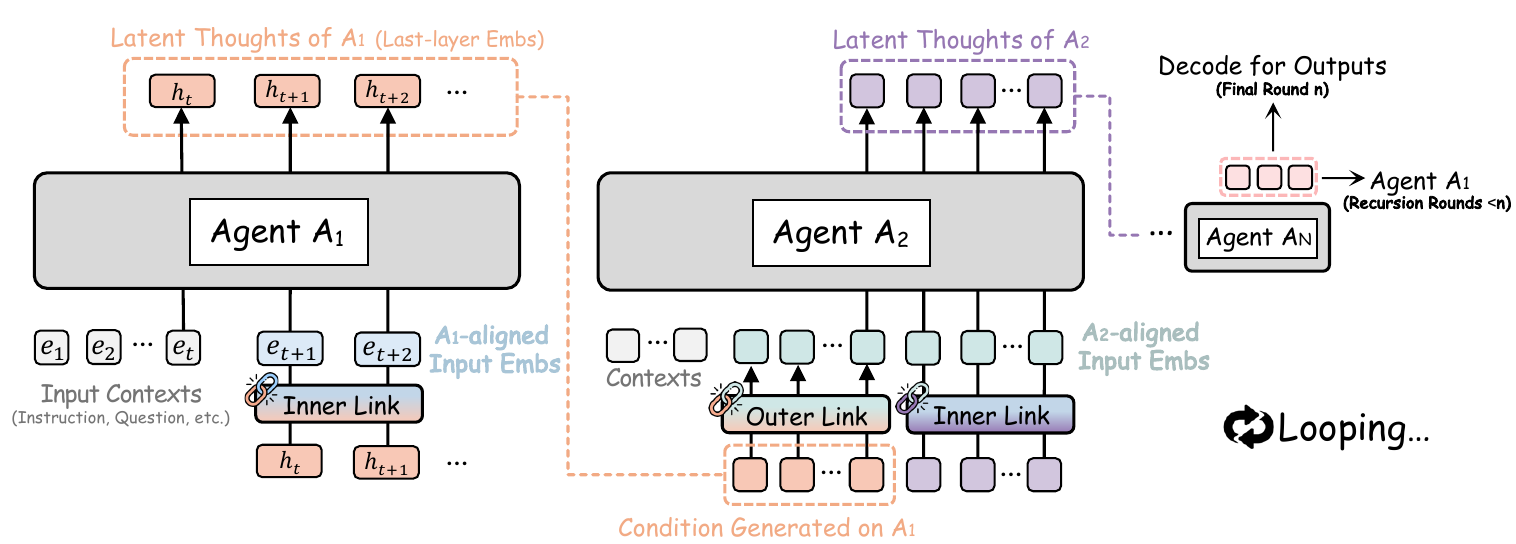
\includegraphics[width=\linewidth,height=0.82\textheight,keepaspectratio]{figures/RecursiveMAS.png}
\end{frame}

\begin{frame}{RecursiveLink}
\centering
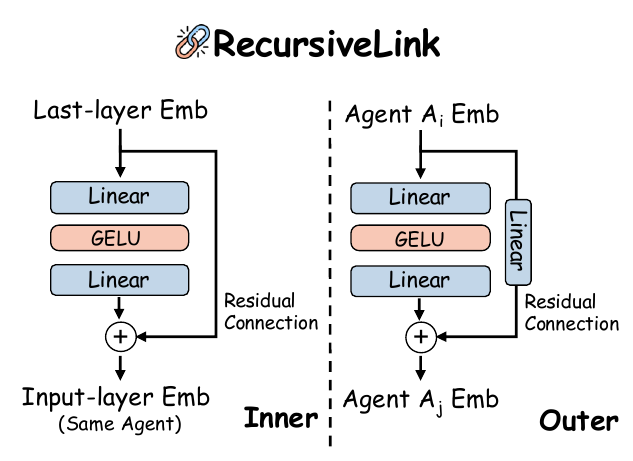
\includegraphics[width=\linewidth,height=0.82\textheight,keepaspectratio]{figures/RecursiveLink.png}
\end{frame}

\begin{frame}{Cache-to-Cache: pairwise cache fusion}
\small
\begin{block}{C2C의 핵심 수식}
\[
C_F^n
=C_R^n(X)+F_n\!\left(C_R^n(X),\,C_S^{G(n)}(X)\right)
\]
\[
y_{i+1}=P\!\left(y_i \mid C_F(X)\oplus C(Y_{0:i})\right)
\]
\end{block}

\vspace{0.3em}
\begin{center}
\begin{tikzpicture}[node distance=0.75cm]
\node[box, minimum width=2.5cm] (s) {Sharer KV};
\node[box, minimum width=2.5cm, below=0.8cm of s] (r) {Receiver KV};
\node[purplebox, minimum width=2.5cm, right=1.0cm of s, yshift=-0.4cm] (f) {Fuser\\\scriptsize projection + gate};
\node[greenbox, minimum width=2.5cm, right=1.0cm of f] (out) {Fused KV};
\draw[arrow] (s) -- (f);
\draw[arrow] (r) -- (f);
\draw[arrow] (f) -- (out);
\end{tikzpicture}
\end{center}

\vspace{0.2em}
\scriptsize
C2C는 receiver가 이미 같은 input \(X\)를 prefill해서 만든 cache를 가지고 있고, 여기에 sharer cache를 residual하게 섞는 구조다.
\end{frame}

\begin{frame}[plain]
\vspace*{0.25em}
\noindent\makebox[0pt][l]{%
\hspace*{-0.065\paperwidth}%

\includegraphics[height=0.82\paperheight,keepaspectratio]{figures/C2C.png}\hspace{0.002\paperwidth}%

\includegraphics[height=0.82\paperheight,keepaspectratio]{figures/LCF.png}%
}
\end{frame}

\begin{frame}{See What I See: dense heterogeneous KV alignment}
\small
\begin{center}
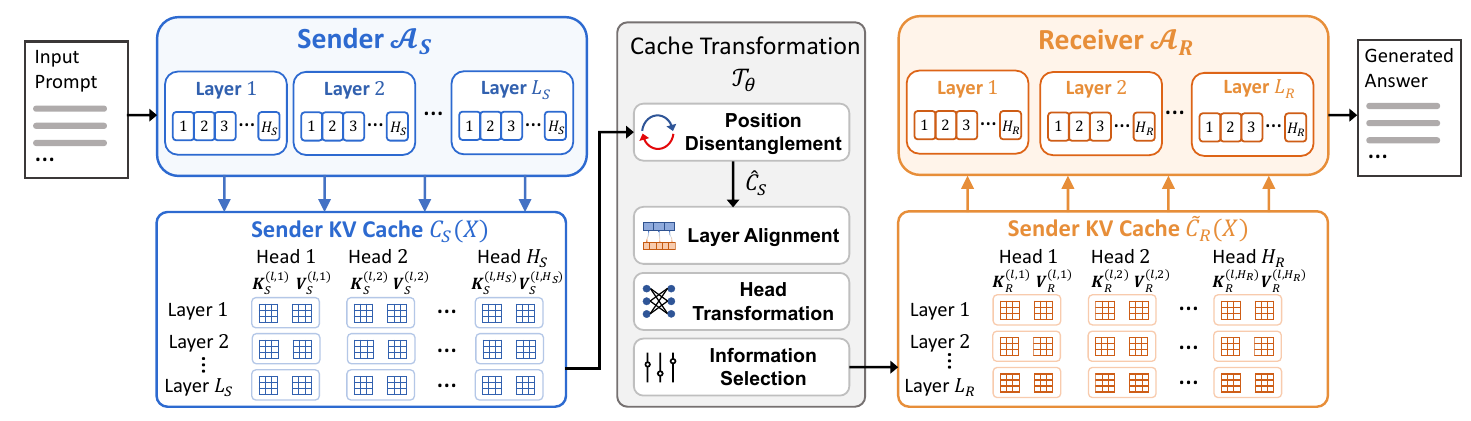
\includegraphics[width=\linewidth,height=0.58\textheight,keepaspectratio]{figures/See what i see.png}
\end{center}

\vspace{-0.2em}
\begin{columns}[T,onlytextwidth]
\column{0.48\textwidth}
\begin{block}{Phase 1: reconstruction}
\scriptsize
Sender와 receiver에 같은 프롬프트를 넣어 각각 KV를 만든다.
Adapter는 sender KV를 receiver가 만들었을 KV처럼 맞추도록 학습한다.
\end{block}

\column{0.48\textwidth}
\begin{block}{Phase 2: generation}
\scriptsize
맞춘 KV를 receiver의 past cache로 실제 주입한다.
이제 ``모양만 비슷한 KV''가 아니라 답 생성에 도움이 되는 KV가 되도록 CE로 학습한다.
\end{block}
\end{columns}

\vspace{0.3em}
\begin{block}{한계}
\scriptsize
Dense KV alignment는 강하지만, 기본 단위는 same-source-context cache translation이다.
Role-conditioned latent thought handoff는 별도 문제로 남는다.
\end{block}
\end{frame}

\begin{frame}{C2C에서 fusion을 쓰는 이유}
\small
\begin{columns}[T,onlytextwidth]
\column{0.48\textwidth}
\begin{block}{왜 receiver KV를 같이 보나?}
\begin{itemize}
  \item Sharer와 Receiver가 같은 context \(X\)를 인코딩한다.
  \item Receiver의 기존 이해를 보존해야 한다.
  \item Gate가 도움이 되는 layer만 선택한다.
\end{itemize}
\end{block}

\column{0.48\textwidth}
\begin{block}{우리 설정과 다른 점}
\begin{itemize}
  \item agent마다 role prompt와 objective가 다르다.
  \item Receiver KV를 만들려면 receiver prefill을 먼저 해야 한다.
  \item 우리는 receiver prefill 전에 prefix memory를 주입하고 싶다.
\end{itemize}
\end{block}
\end{columns}

\vspace{0.7em}
\begin{block}{}
\small
따라서 HeteroMAS는 C2C-style fusion이 아니라 \textbf{sender-only KV translation + prefix prepend}를 기본 구조로 둔다.
\end{block}
\end{frame}

\begin{frame}{현재 Heterogeneous KV 연구들의 한계}
\small
\begin{columns}[T,onlytextwidth]
\column{0.48\textwidth}
\begin{block}{무엇을 잘하나}
\begin{itemize}
  \item 서로 다른 모델의 KV cache shape을 맞춘다.
  \item sender cache를 receiver-native cache로 번역한다.
  \item text decode/re-encode 비용을 줄인다.
\end{itemize}
\end{block}

\column{0.48\textwidth}
\begin{block}{무엇이 빠져 있나}
\begin{itemize}
  \item sender가 role-conditioned \term{latent thought}를 생성하지 않는다.
  \item 같은 source context \(X\)의 cache alignment에 가깝다.
  \item MAS의 planner \(\rightarrow\) refiner \(\rightarrow\) solver handoff를 직접 모델링하지 않는다.
\end{itemize}
\end{block}
\end{columns}

\vspace{0.8em}
\begin{center}
\begin{tikzpicture}[node distance=0.75cm]
\node[box, minimum width=3.2cm] (cache) {Existing Hetero KV\\\scriptsize \(C_S(X)\rightarrow \tilde C_R(X)\)};
\node[redbox, minimum width=2.8cm, right=0.9cm of cache] (gap) {Missing\\\scriptsize latent thought};
\node[greenbox, minimum width=3.2cm, right=0.9cm of gap] (mas) {Target MAS Handoff\\\scriptsize \(C_{\mathrm{think}}\rightarrow\) role slot};
\draw[arrow] (cache) -- (gap);
\draw[arrow] (gap) -- (mas);
\end{tikzpicture}
\end{center}

\vspace{0.5em}
\begin{block}{핵심 문제}
\small
기존 heterogeneous KV transfer는 ``내가 본 context를 네 cache로 바꾼다''에 가깝고,
우리가 필요한 것은 ``내가 agent role에서 생각한 latent state를 네 role의 communication slot으로 넘긴다''이다.
\end{block}
\end{frame}
